%Version 3 October 2023
% See section 11 of the User Manual for version history
%
%%%%%%%%%%%%%%%%%%%%%%%%%%%%%%%%%%%%%%%%%%%%%%%%%%%%%%%%%%%%%%%%%%%%%%
%%                                                                 %%
%% Please do not use \input{...} to include other tex files.       %%
%% Submit your LaTeX manuscript as one .tex document.              %%
%%                                                                 %%
%% All additional figures and files should be attached             %%
%% separately and not embedded in the \TeX\ document itself.       %%
%%                                                                 %%
%%%%%%%%%%%%%%%%%%%%%%%%%%%%%%%%%%%%%%%%%%%%%%%%%%%%%%%%%%%%%%%%%%%%%

%%\documentclass[referee,sn-basic]{sn-jnl}% referee option is meant for double line spacing

%%=======================================================%%
%% to print line numbers in the margin use lineno option %%
%%=======================================================%%

\documentclass{sn-jnl}% Basic Springer Nature Reference Style/Chemistry Reference Style

%%======================================================%%
%% to compile with pdflatex/xelatex use pdflatex option %%
%%======================================================%%

%%\documentclass[pdflatex,sn-basic]{sn-jnl}% Basic Springer Nature Reference Style/Chemistry Reference Style


%%Note: the following reference styles support Namedate and Numbered referencing. By default the style follows the most common style. To switch between the options you can add or remove “Numbered” in the optional parenthesis. 
%%The option is available for: sn-basic.bst, sn-vancouver.bst, sn-chicago.bst%  
 
%%\documentclass[sn-nature]{sn-jnl}% Style for submissions to Nature Portfolio journals
%%\documentclass[sn-basic]{sn-jnl}% Basic Springer Nature Reference Style/Chemistry Reference Style
% \documentclass[sn-mathphys-num]{sn-jnl}% Math and Physical Sciences Numbered Reference Style 
%%\documentclass[sn-mathphys-ay]{sn-jnl}% Math and Physical Sciences Author Year Reference Style
%%\documentclass[sn-aps]{sn-jnl}% American Physical Society (APS) Reference Style
%%\documentclass[sn-vancouver,Numbered]{sn-jnl}% Vancouver Reference Style
%%\documentclass[sn-apa]{sn-jnl}% APA Reference Style 
%%\documentclass[sn-chicago]{sn-jnl}% Chicago-based Humanities Reference Style

%%%% Standard Packages
%%<additional latex packages if required can be included here>


\usepackage{graphicx}%
\usepackage{multirow}%
\usepackage{amsmath,amssymb,amsfonts}%
\usepackage{amsthm}%
\usepackage{mathrsfs}%
\usepackage[title]{appendix}%
\usepackage{xcolor}%
\usepackage{textcomp}%
\usepackage{manyfoot}%
\usepackage{booktabs}%
\usepackage{algorithm}%
\usepackage{algorithmicx}%
\usepackage{algpseudocode}%
\usepackage{listings}%
\usepackage{comment} % 
\usepackage{graphicx}
% \RequirePackage{mathptmx}      % use Times fonts if available on your TeX system
% \RequirePackage{flushend}
% \RequirePackage[numbers,sort&compress]{natbib}
% \RequirePackage[colorlinks,citecolor=blue,urlcolor=blue,linkcolor=blue]{hyperref}
\usepackage{subcaption}
\usepackage{array}
\usepackage{pgf-umlsd}
\usepackage{makecell}
\usepackage[usestackEOL]{stackengine}
\usepackage{cite}
%%%%

%%%%%=============================================================================%%%%
%%%%  Remarks: This template is provided to aid authors with the preparation
%%%%  of original research articles intended for submission to journals published 
%%%%  by Springer Nature. The guidance has been prepared in partnership with 
%%%%  production teams to conform to Springer Nature technical requirements. 
%%%%  Editorial and presentation requirements differ among journal portfolios and 
%%%%  research disciplines. You may find sections in this template are irrelevant 
%%%%  to your work and are empowered to omit any such section if allowed by the 
%%%%  journal you intend to submit to. The submission guidelines and policies 
%%%%  of the journal take precedence. A detailed User Manual is available in the 
%%%%  template package for technical guidance.
%%%%%=============================================================================%%%%

% %% as per the requirement new theorem styles can be included as shown below
% \theoremstyle{thmstyleone}%
% \newtheorem{theorem}{Theorem}%  meant for continuous numbers
% %%\newtheorem{theorem}{Theorem}[section]% meant for sectionwise numbers
% %% optional argument [theorem] produces theorem numbering sequence instead of independent numbers for Proposition
% \newtheorem{proposition}[theorem]{Proposition}% 
% %%\newtheorem{proposition}{Proposition}% to get separate numbers for theorem and proposition etc.

% \theoremstyle{thmstyletwo}%
% \newtheorem{example}{Example}%
% \newtheorem{remark}{Remark}%

% \theoremstyle{thmstylethree}%
% \newtheorem{definition}{Definition}%

\raggedbottom
%%\unnumbered% uncomment this for unnumbered level heads

\begin{document}

\title[Article Title]{BORTNET: Borda-based Resilient Trust Network Evaluation in Fog}

%%=============================================================%%
%% GivenName	-> \fnm{Joergen W.}
%% Particle	-> \spfx{van der} -> surname prefix
%% FamilyName	-> \sur{Ploeg}
%% Suffix	-> \sfx{IV}
%% \author*[1,2]{\fnm{Joergen W.} \spfx{van der} \sur{Ploeg} 
%%  \sfx{IV}}\email{iauthor@gmail.com}
%%=============================================================%%

\author*[1]{\fnm{Rasagna} \sur{V}}\email{p20200019@hyderabad.bits-pilani.ac.in}

\author[1]{\fnm{Geethakumari} \sur{G}}\email{geetha@hyderabad.bits-pilani.ac.in}
% \equalcont{These authors contributed equally to this work.}

\author[1]{\fnm{Timothy} \sur{B}}\email{f20212978@hyderabad.bits-pilani.ac.in}
% \equalcont{These authors contributed equally to this work.}
\author[1]{\fnm{ SriPada } \sur{J}}\email{f20212813@hyderabad.bits-pilani.ac.in}

% \equalcont{These authors contributed equally to this work.}

\affil[1]{
\orgname{Birla Institute of Technology and Science}, \orgaddress{\city{Hyderabad Campus}, \country{India}}}

% \affil[2]{\orgdiv{CSIS},
% \orgname{BITS Pilani}, \orgaddress{\street{Shamirpet}, \city{Hyderabad Campus}, \postcode{500078}, \state{Telangana}, \country{India}}}


% \affil[2]{\orgdiv{Dept of EEE},
% \orgname{Birla Institute of Technology and Science}, \orgaddress{\city{Hyderabad Campus}, \country{India}}}


% \affil[4]{\orgdiv{CSIS},
% \orgname{BITS Pilani}, \orgaddress{\street{Shamirpet}, \city{Hyderabad Campus}, \postcode{500078}, \state{Telangana}, \country{India}}}


%%==================================%%
%% Sample for unstructured abstract %%
%%==================================%%

\abstract{Fog computing extends cloud services to network edges, facilitating real-time processing and low latency. However, its decentralized nature introduces security challenges, including trust-based attacks like ballot stuffing. Ballot stuffing manipulates decision outcomes by injecting biased votes, posing a significant threat in fog environments. Traditional security measures are often inadequate in countering such attacks. To address this, the Borda scoring method emerges as a promising solution. Derived from social choice theory, Borda assigns scores based on option rankings in each ballot, providing a resilient mechanism against manipulation. It functions as a consensus mechanism, aggregating opinions from all nodes in the network to ensure fair decision-making. Integrating Borda scoring into fog computing mitigates trust-based attacks like ballot stuffing, enhancing decision-making reliability and security.}

%%================================%%
%% Sample for structured abstract %%
%%================================%%

% \abstract{\textbf{Purpose:} The abstract serves both as a general introduction to the topic and as a brief, non-technical summary of the main results and their implications. The abstract must not include subheadings (unless expressly permitted in the journal's Instructions to Authors), equations or citations. As a guide the abstract should not exceed 200 words. Most journals do not set a hard limit however authors are advised to check the author instructions for the journal they are submitting to.
% 
% \textbf{Methods:} The abstract serves both as a general introduction to the topic and as a brief, non-technical summary of the main results and their implications. The abstract must not include subheadings (unless expressly permitted in the journal's Instructions to Authors), equations or citations. As a guide the abstract should not exceed 200 words. Most journals do not set a hard limit however authors are advised to check the author instructions for the journal they are submitting to.
% 
% \textbf{Results:} The abstract serves both as a general introduction to the topic and as a brief, non-technical summary of the main results and their implications. The abstract must not include subheadings (unless expressly permitted in the journal's Instructions to Authors), equations or citations. As a guide the abstract should not exceed 200 words. Most journals do not set a hard limit however authors are advised to check the author instructions for the journal they are submitting to.
% 
% \textbf{Conclusion:} The abstract serves both as a general introduction to the topic and as a brief, non-technical summary of the main results and their implications. The abstract must not include subheadings (unless expressly permitted in the journal's Instructions to Authors), equations or citations. As a guide the abstract should not exceed 200 words. Most journals do not set a hard limit however authors are advised to check the author instructions for the journal they are submitting to.}

\keywords{Fog Computing, Trust Based Attacks, Ballot Stuffing, Borda Scoring}

%%\pacs[JEL Classification]{D8, H51}

%%\pacs[MSC Classification]{35A01, 65L10, 65L12, 65L20, 65L70}

\maketitle


\section{Introduction}
Fog computing has emerged as a transformative shift in distributed computing, extending the capabilities of cloud services to the edge of the network. Unlike traditional cloud computing, where data processing is centralized in distant data centers, fog computing decentralizes these processes, bringing computing resources closer to where data is generated. 

% This proximity enables real-time processing, reduces latency, and improves efficiency—making fog computing ideal for time-sensitive applications such as the Internet of Things (IoT), smart cities, and autonomous systems\cite{bonomi2012fog,chiang2016fog}. 

However, the distributed nature of fog computing introduces new security challenges that necessitate innovative approaches to ensure the integrity, confidentiality, and reliability of data and operations \cite{yi2015survey}.

Security in fog computing encompasses various aspects, including data privacy, integrity, availability, and trustworthiness. Since data processing and storage are distributed across a vast network of edge devices, securing these resources against unauthorized access, data breaches, and malicious activities becomes critical. Additionally, the dynamic nature of fog environments, characterized by frequent device mobility and network topology changes, complicates security management \cite{mao2017survey}. As a result, ensuring the secure operation of fog networks requires solutions that are adaptable to the fluidity of the environment.

Among the many security threats that fog computing faces, trust-based attacks stand out as particularly concerning. These attacks exploit vulnerabilities within the trust relationships established between nodes in the fog network, potentially compromising decision-making processes and eroding the system's trustworthiness \cite{junejo2019trustee}. Various forms of trust-based attacks, such as bad mouthing, good mouthing, on-off attacks, ballot stuffing, self-promotion, and whitewashing, can severely impact the reliability of fog networks. In particular, ballot stuffing attacks are a significant threat, where malicious nodes inject biased or fake votes into the decision-making process, manipulating the outcomes to favor a specific result \cite{nair2023ai}.

Mitigating ballot stuffing attacks in fog computing is critical for preserving the integrity of decision-making processes, especially in applications where compromised decisions can have serious consequences, such as in healthcare, autonomous vehicles, and critical infrastructure. In a fog environment, malicious nodes can exploit system vulnerabilities to conduct ballot stuffing attacks, skewing decision outcomes and undermining the network's overall trust. Given the increasing deployment of IoT devices and other edge technologies in fog networks, the potential for such manipulations is heightened, making it imperative to develop robust countermeasures. Effective mitigation not only protects individual systems from attack but also ensures the overall security, integrity, and trustworthiness of the fog computing ecosystem.

In this paper, we focus on addressing the ballot stuffing attack in fog computing. We propose an approach based on the Borda scoring method, which offers a resilient mechanism for mitigating trust-based manipulations in distributed decision-making processes. Derived from social choice theory, the Borda method provides a score-based ranking system that can aggregate opinions from multiple nodes, ensuring fair decision-making even in the presence of malicious actors. By integrating this method into the security architecture of fog networks, we aim to enhance the system's resistance to ballot stuffing attacks and improve the reliability of fog-based decision-making processes.
\section{Related Work}
In recent years, the need for trust-based security solutions in fog computing has gained significant attention in both academic and industrial spheres. As networks become more decentralized, especially with the rise of the Internet of Things (IoT), the security of these systems becomes a critical concern. Trust plays a crucial role in such environments, acting as a method to identify and isolate malicious nodes by leveraging interactions with legitimate nodes. Trust-based systems can foster strong relationships among fog nodes, ensuring both privacy and security are maintained across the network\cite{wang2013internet}.
One of the major challenges in designing trust management mechanisms for fog nodes arises from the decentralized nature of fog computing environments. Traditional centralized trust systems are not suitable due to the inherent architecture of fog computing, where data and computational tasks are distributed across various fog nodes rather than being handled by a single entity. This decentralization complicates the collection and management of necessary evidence—such as behavior logs, communication history, or feedback—to accurately evaluate the trustworthiness of distributed fog nodes\cite{ni2017securing}.Moreover, these trust-based systems must operate efficiently in dynamic environments, where nodes frequently join or leave the network, and potential threats continuously evolve.

In one study, the authors calculated the trustworthiness of fog service providers using a variety of trust metrics, including reliability, security, feedback, and cost. While this multi-faceted evaluation provided a comprehensive overview of trust in the system, a key assumption of the study was the honesty of user feedback. Trust-based attacks, such as ballot stuffing (where malicious nodes submit false feedback to increase their trust scores), were recognized as a potential threat, but the study did not provide explicit mechanisms to address such attacks \cite{rahman2020find}.This limitation underscores the need for more robust solutions capable of identifying and mitigating dishonest behavior from malicious nodes.
Other researchers have adopted subjective logic mechanisms to enhance trust evaluation in fog computing environments. Subjective logic is a probabilistic approach that allows trust to be modeled with a degree of uncertainty, which is especially useful in environments like fog computing where complete information is rarely available. However, while subjective logic can be effective for detecting trust-based attacks, the specifics of mitigating ballot stuffing were not detailed in these studies\cite{al2021subjective}.
In another method, a multi-source trust evaluation approach was proposed to identify malicious nodes in fog computing systems. This method calculated the final trust score of IoT devices by using a weighted sum of experiences from fog nodes and trust level values from neighboring nodes. A key feature of this approach was the use of the PageRank algorithm to prioritize trust level values from reputable neighbors. However, the assumption that all neighboring fog nodes are trustworthy introduces potential vulnerabilities, as malicious nodes could still influence trust scores. If the final trust value of an IoT device fell below a certain threshold, the device would be flagged as malicious. Despite its merits, the method was limited by the risk of relying on potentially malicious trust values from neighboring nodes, highlighting the necessity of assessing the credibility of such sources \cite{hussain2018trfiot,hussain2020context}
Another noteworthy approach, known as CTRUST, incorporates a belief function to assess a node's concurrence with recommendations from third-party nodes. The belief function offers a way to measure confidence in the trustworthiness of another node based on the recommendations it receives. Although the CTRUST framework provides a structured mechanism for trust evaluation, it focuses heavily on quantitative analysis and neglects to address the inherent imprecision and uncertainty present in fog environments. Additionally, CTRUST does not address critical attack vectors like ballot stuffing, leaving a gap in its overall security coverage \cite{adewuyi2019ctrust},

In an attempt to mitigate some of these challenges, researchers introduced a hierarchical trust model designed specifically for sensor-to-cloud applications utilizing fog computing. This model enables wireless sensor nodes to establish trust relationships not only with one another but also with cloud service providers and other sensor service providers (fog providers). The hierarchical structure of this model is intended to facilitate efficient detection of malicious nodes while reducing energy consumption. The system also aims to recover nodes affected by various attacks such as bad-mouthing, good-mouthing, and ballot stuffing attacks. Despite the advantages of this hierarchical structure, the authors did not provide specific strategies to mitigate ballot stuffing attacks, which remain a critical vulnerability in such environments \cite{wang2020novel}.
As fog computing continues to grow in complexity and scale, trust-based security systems must evolve to address both new and existing challenges. While significant progress has been made in developing methods for trust evaluation, critical issues—particularly concerning trust-based attacks like ballot stuffing—are still inadequately addressed. Future research should focus on refining these systems to account for both the dynamic nature of fog computing environments and the potential for malicious behavior from both internal and external nodes.
\section{Preliminaries}
\subsection{Ballot Stuffing Attack}

Ballot stuffing attacks in fog computing, analogous to malicious nodes, pose a significant threat to the integrity and reliability of decision-making processes within the network. In traditional ballot stuffing, malicious actors illegitimately influence the outcome of an election by fraudulently casting multiple votes or manipulating the vote count. Similarly, in fog computing, malicious nodes attempt to subvert the decision-making process by dishonestly influencing the aggregation of trust or preference ratings, thereby compromising the accuracy and trustworthiness of decisions. A typical ballot stuffing attack has been depicted in Fig. \ref{fig_1}. The figure shows a Fog Manager Node that collects votes from both genuine and malicious fog nodes. The malicious nodes send malicious votes, trying to manipulate the final decision. The Fog Manager's job is to collect, validate, and process these votes to ensure an accurate and fair decision, but in the presence of ballot stuffing (from malicious nodes), the results could be skewed if proper validation measures are not in place.
\begin{figure}[h!]
\begin{center}
\frame{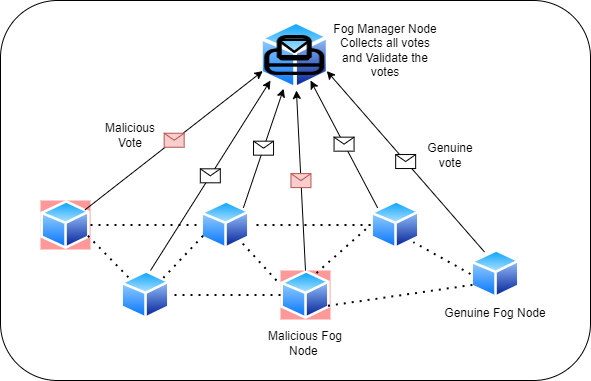
\includegraphics[width=0.95\linewidth]{bst/images/ballot_attack.drawio.png}}
\caption{A Simple Ballot Stuffing Attack Scenario.}
\label{fig_1}
\end{center}

\end{figure}


The consequences of ballot stuffing attacks in fog computing can be severe, particularly in safety-critical applications or environments where decisions impact human safety or operational integrity. For example, in a smart city deployment relying on fog computing for traffic management, a malicious node orchestrating a ballot stuffing attack could manipulate traffic signal timings, leading to congestion, accidents, or other adverse consequences.
\subsection{Borda scoring}
Borda scoring is a preferential voting method utilized to determine the collective preference or ranking of a set of options based on individual preferences or rankings. It was first proposed by the French mathematician Jean-Charles de Borda in the 18th century and has since found applications in various decision-making processes, including elections, ranking systems, and consensus-building mechanisms.
The fundamental principle behind Borda scoring is to assign scores to each option based on its ranking by individuals. In a typical Borda scoring system, the highest-ranked option receives the maximum score, while the lowest-ranked option receives the minimum score. The scores assigned to intermediate rankings are determined by a predefined scoring scheme, often following an arithmetic progression.
For example, in a scenario with \( n \) options, the highest-ranked option would receive a score of \( n \), the second-highest-ranked option would receive a score of \( n-1 \), and so forth, with the lowest-ranked option receiving a score of 1. Once individual rankings are collected, the scores assigned to each option are aggregated across all participants to calculate the total score for each option. The option with the highest total score is deemed the most preferred or ranked the highest by the collective group.


Borda scoring is particularly advantageous due to its ability to capture nuanced preferences and provide a comprehensive ranking of options, even in situations with multiple alternatives and diverse individual opinions. It promotes fairness and transparency by considering all preferences and mitigating the influence of outliers or individual biases.
Utilizing Borda Scoring Method to prevent Ballot Stuffing Attack :
In the context of fog computing and decision-making processes, Borda scoring can be applied to assess the trustworthiness or reliability of nodes based on their interactions and perceived trust levels. By aggregating trust ratings from multiple sources using Borda scoring, a comprehensive assessment of node trustworthiness can be obtained, facilitating informed decision-making and enhancing the security and resilience of fog computing systems.
bei
\subsubsection*{Utilizing Borda Scoring Method to prevent Ballot Stuffing Attack}


In the context of fog computing and decision-making processes, Borda scoring can be applied to assess the trustworthiness or reliability of nodes based on their interactions and perceived trust levels. By aggregating trust ratings from multiple sources using Borda scoring, a comprehensive assessment of node trustworthiness can be obtained, facilitating informed decision-making and enhancing the security and resilience of fog computing systems.
% \begin{table*}[ht!]
% \centering
% \caption{Node Rankings and Borda Points}
% \label{tab:node_rankings}
% \begin{tabular}{|c|c|c|c|c|c|c|}
% \hline
% \textbf{Node} & \textbf{P1 Ranking} & \textbf{P1 Points} & \textbf{P2 Ranking} & \textbf{P2 Points} & \textbf{P3 Ranking} & \textbf{P3 Points} \\ 
% \hline
% Node A & 1st & 3 points & 2nd & 2 points & 3rd & 1 point \\ \hline
% Node B & 3rd & 1 point & 1st & 3 points & 2nd & 2 points \\ \hline
% Node C & 2nd & 2 points & 3rd & 1 point & 1st & 3 points \\ \hline
% \end{tabular}

% \end{table*}
\begin{comment}
\begin{table*}[ht!]
\centering
\caption{Node Rankings and Borda Points}
\label{tab:node_rankings}
\resizebox{\textwidth}{!}{  % Resize to the text width, maintaining aspect ratio
\begin{tabular}{|c|c|c|c|c|c|c|}
\hline
\textbf{Node} & \textbf{P1 Ranking} & \textbf{P1 Points} & \textbf{P2 Ranking} & \textbf{P2 Points} & \textbf{P3 Ranking} & \textbf{P3 Points} \\ 
\hline
Node A & 1st & 3 points & 2nd & 2 points & 3rd & 1 point \\ \hline
Node B & 3rd & 1 point & 1st & 3 points & 2nd & 2 points \\ \hline
Node C & 2nd & 2 points & 3rd & 1 point & 1st & 3 points \\ \hline
\end{tabular}
}
\end{table*}

\begin{table}[h!]
\centering
\caption{Total Borda Scores for Each Proposal}
\label{tab:point_rankings}
\begin{tabular}{|c|c|}
\hline
\textbf{Proposal} & \textbf{Total Borda Points} \\ \hline
P1 & 3 + 2 + 1 = 6 points \\ \hline
P2 & 2 + 3 + 2 = 7 points \\ \hline
P3 & 1 + 1 + 3 = 5 points \\ \hline
\end{tabular}

\end{table}
\subsection*{Borda Scoring Example}

Consider a network of three nodes (Node A, Node B, and Node C) that need to decide on one of three proposals: \( P_1, P_2, P_3 \). Each node ranks the proposals in order of preference. In Borda scoring, the first choice gets the most points, the second gets fewer, and so on as described in Table \ref{tab:node_rankings}. Node A ranks its proposal P1 first followed by P2 and P3. Hence points allocated for these proposals with 3, 2 and 1 respectively. Similarly Node B and Node C will also allocate their respective points.




We now calculate the total Borda scores for each proposal. The total score for each proposal is the sum of the points assigned by each node as shown in Table \ref{tab:point_rankings}.




After aggregating the Borda points, we find the following total scores:

\begin{itemize}
    \item P1: 6 points
    \item P2: 7 points
    \item P3: 5 points
\end{itemize}

Based on the highest Borda score, \textbf{P2} is the winning proposal with 7 points. Borda scoring provides an effective method for aggregating preferences in fog networks. By assigning points based on rankings, Borda scoring helps select the most preferred option, in this case, proposal \( P_2 \). The method ensures a fair decision-making process and can be used to improve consensus in decentralized environments.
\end{comment}
% \section{Proposed BOMBAT Approach}
% Our methodology focuses on enhancing the integrity and trustworthiness of decision-making processes within the fog network, thereby safeguarding against potential manipulation and ensuring the reliability of critical operations. By leveraging techniques such as direct trust calculation, Borda scoring, and proactive detection mechanisms, we aim to detect, analyze, and mitigate instances of ballot stuffing before they can inflict harm. Through this proactive stance, we seek to fortify the resilience of fog computing systems, particularly in safety-critical applications where the consequences of manipulation can have far-reaching implications for human safety and operational integrity.

% We introduce a solution called BOMBAT  to mitigate Ballot stuffing Attacks in Fog computing System. The fog nodes communicate among themselves in the fog environment to process the data. Acting as a central coordinator, the fog manager orchestrates and monitors the activities of all nodes within the network, ensuring seamless operation and coordination.
% The fog manager observes the communication between nodes and computes the direct trust values among the nodes in the network. Direct trust represents the level of confidence or reliance that one node has in another within the network. Direct trust in our approach is calculated by examining packet transfer metrics, with the level of trust represented on a scale from 0 to 1, where 0 signifies no trust and 1 represents complete trust. For example if a node has a direct trust value of 0.5 it means that the node is sending 50\% of the packets and dropping off the other 50\% of the packets. Each node's direct trust is calculated by the fog manager and stored in the Trust Matrix. Once the trust matrix is generated, we employ the Borda scoring method to assign scores to each node based on its perceived trustworthiness. These scores are determined by the fog manager using the trust values stored in the matrix. Subsequently, each node is tasked with ranking all other nodes based on their direct interactions, reflecting their individual experiences and perceptions of trust. Following this, we compare the total Borda scores obtained from node rankings with the initial scores assigned by the fog manager. This step serves to identify any significant discrepancies or violations in the rankings, potentially indicative of attempts to manipulate the system.
% To detect and address such violations, we scrutinize the before and after rankings of each node to compile a suspect list of nodes exhibiting suspicious behavior. By comparing the initial Borda scores assigned by the fog manager with the updated scores derived from node rankings, we can pinpoint any discrepancies suggestive of potential ballot stuffing attacks or manipulation attempts. The nodes appearing most frequently on the suspect list are flagged as the most suspicious and subjected to further analysis. To mitigate the risks posed by these suspicious nodes, we implement a removal mechanism, whereby the node with the highest frequency of appearance in the suspect list is removed from the network. This proactive measure aims to prevent the propagation of malicious influence and preserve the integrity of decision-making processes within the fog computing environment. Through this comprehensive approach, we can effectively detect, analyze, and mitigate violations in rankings, thereby enhancing the resilience of the fog computing system against ballot stuffing attacks and ensuring the trustworthiness of decision-making processes.


\section{Proposed BORTNET Methodology}
Our methodology is formulated to identify rogue nodes within a fog computing environment systematically. This is accomplished through a series of defined steps, starting with the computation of trust matrices, followed by the analysis of node behavior through voting matrices, and culminating in a systematic identification of potential rogue nodes. Each phase of the proposed methodology is described below.

\subsection{Computation of Trust Matrix}

The methodology initiates with the generation of a trust matrix $T$ by the fog manager, modeling the network with a star topology where each node is directly connected to every other node. The trust values for each node are initialized at a baseline level, and the system simulates multiple rounds of node interactions, adjusting trust scores based on the outcomes of these interactions. This simulation helps in establishing a comprehensive trust matrix that encapsulates the trustworthiness of each node.



\subsection{Identification and Management of Rogue Nodes}

In adherence to the principles of Byzantine fault tolerance, the system constrains the number of rogue nodes to a fraction of the total nodes to ensure network integrity. A scenario is set up where certain nodes are hypothesized as rogue to demonstrate the detection process. The system employs methods to identify discrepancies that could indicate manipulations typical of rogue nodes.

\subsection{Populating and Analyzing the Voting Matrix}

The fog manager initially employs a ranking method to evaluate nodes based on their performance metrics, documented in a voting matrix $B$. In the event of manipulation, a secondary manipulated voting matrix $B'$ is produced, reflecting the distorted rankings. By comparing the original and manipulated matrices, potential attacks are identified. This comparison is pivotal for determining whether shifts in node rankings represent genuine security threats.

\subsection{Systematic Identification of Rogue Nodes}

Following the identification of rank discrepancies, a suspect matrix is formulated, listing all nodes along with the rank changes they induce in others. A scoring system evaluates each node based on the magnitude of these changes, disregarding the direction of change. Nodes with the highest cumulative scores are flagged as potential rogues, indicating a high probability of disruptive behavior.

\subsection{Periodic Monitoring and Reevaluation}

The methodology emphasizes the need for periodic monitoring and reevaluation to maintain network integrity. Stable networks show consistent node rankings over time, while the emergence of new discrepancies could signal potential security threats. This ongoing assessment is crucial for adapting to new threats and maintaining the operational efficacy of the system.

This structured and iterative approach ensures continuous monitoring and the robust detection of rogue nodes, thereby safeguarding the network against internal disruptions and external attacks.
\begin{algorithm}
\caption{ Proposed Borda-based Resilient Trust Network Evaluation in Fog Algorithm (BORTNET) }
\begin{algorithmic}[1]
\State \textbf{Input:} Nodes $N$, Initial trust level $\tau_{init}$
\State \textbf{Output:} List of rogue nodes $R$

\Procedure{ComputeTrust}{$N$, $\tau_{init}$}
    \State Initialize trust matrix $T$ with $\tau_{init}$
    \For{$i \gets 1$ to $num\_rounds$}
        \State Simulate communication, update $T$
    \EndFor
    \State \Return $T$
\EndProcedure

\Procedure{DetectRogues}{$T$}
    \State Initialize Borda count $B$ and manipulated Borda $B'$
    \State $B \gets$ Rank nodes based on $T$
    \State $B' \gets$ Simulate attack, manipulate $B$
    \State Calculate discrepancies $D$ between $B$ and $B'$
    \State \Return Nodes with significant discrepancies in $D$
\EndProcedure

\Procedure{CalculateScores}{$D$}
    \State Initialize score vector $S$
    \For{each $n \in N$}
        \State $S[n] \gets$ Sum of discrepancies affecting $n$
    \EndFor
    \State Sort $N$ by $S$, identify top suspects in $R$
    \State \Return $R$
\EndProcedure

\Procedure{Main}{}
    \State $T \gets$ \Call{ComputeTrust}{$N$, $\tau_{init}$}
    \State $suspects \gets$ \Call{DetectRogues}{$T$}
    \State $rogueNodes \gets$ \Call{CalculateScores}{$suspects$}
    \State \Return $rogueNodes$
\EndProcedure

\end{algorithmic}
\end{algorithm}


\section{Experimental Results}
The subsequent paragraphs detail various settings and the results achieved at each stage of the process undertaken.
\begin{itemize}
\item \textbf{Computation of Trust Matrix:} The initial input for our proposed approach is the trust matrix, which is generated by the fog manager. We model the network as a star topology, enabling each node to communicate with all other nodes directly. The trust values, ranging between 0 and 1, are initially set at 0.5 for each node. We simulate 200 rounds of communication between the nodes using Matlab. During each communication round, there is a randomly assigned 50\% chance for either successful communication or a packet drop. Each successful communication increases a node’s trust score by 0.0025, and similarly, it decreases with each packet drop. After completing 200 rounds, the final trust matrix is obtained. It should be noted that extensive research has been conducted on the generation of trust matrices using various methodologies as described in literature\cite{caminha2018smart,najib2019survey}, and any of these methods could potentially be employed to construct this trust matrix. A sample trust matrix for six nodes is depicted in Fig. \ref{tab:trust_matrix}.

    
\begin{table}[htbp]
\centering
\renewcommand{\arraystretch}{1.5} % Adjusts the row height, increase the number for more space
\caption{Trust Matrix Computation for all the nodes in  the network.}
\label{tab:trust_matrix}
\begin{tabular}{|c|c|c|c|c|c|c|c|}
\hline
\textbf{} & \textbf{N1} & \textbf{N2} & \textbf{N3} & \textbf{N4} & \textbf{N5} & \textbf{N6} & \textbf{N7}\\
\hline
\textbf{N1} & 0.0000 & 0.5250 & 0.5200 & 0.5800 &0.5300 &0.5600 & 0.5750 \\
\hline
\textbf{N2} & 0.5750 & 0.0000 & 0.5500 & 0.5450 & 0.5250 & 0.5350 & 0.5450\\
\hline
\textbf{N3} & 0.5400 &0.5300 & 0.0000 & 0.5250 & 0.4950 & 0.5150 & 0.4650 \\
\hline
\textbf{N4} & 0.5350 & 0.5000 & 0.4750 & 0.0000 & 0.4800 & 0.4950 & 0.5150 \\
\hline
\textbf{N5} & 0.4650 & 0.4450 & 0.4950 & 0.4750 & 0.0000 & 0.4800 & 0.4400\\
\hline
\textbf{N6} & 0.4400 & 0.4750 & 0.5000 & 0.4450 & 0.4750 & 0.0000 & 0.485\\
\hline
\textbf{N7} & 0.395 & 0.4300 & 0.4700 & 0.4500 & 0.4200  & 0.4750 & 0.0000\\
\hline
\end{tabular}
\end{table}


\begin{figure*}[h!]
    \centering
    \scalebox{0.6}{
 \begin{sequencediagram}
    \newthread{fm}{Fog Manager}
    \newinst[2]{tm}{Trust Matrix Gen}
    \newinst[2]{vm}{Voting Matrix Analyzer}
    \newinst[2]{rd}{Rogue Node Detector}

    \begin{call}{fm}{Generate Trust Matrix}{tm}{Trust Matrix}
    \end{call}
    \begin{call}{fm}{Detect Rogue Nodes}{vm}{Discrepancies}
        \begin{call}{vm}{Analyze Voting Matrix}{rd}{Scores}
        \end{call}
    \end{call}
    \begin{call}{fm}{Identify Rogues}{rd}{Rogue Nodes}
    \end{call}
    \begin{sdblock}{Loop}{Periodic Monitoring}
        \begin{call}{fm}{Reassess Network}{fm}{}
        \end{call}
    \end{sdblock}
\end{sequencediagram}
}
\caption{Sequence diagram illustrating the workflow of the proposed BORTNET methodology.}
\end{figure*}
\item \textbf{Number of Rogue Nodes :} According to the Byzantine principle \cite{castro1999practical}, the maximum number of rogue nodes is limited to less than one-third of the total nodes within the system. Thus, in our fog environment comprising seven nodes, a maximum of two rogue nodes is permissible. For this toy example we consider N6 and N7 to be rogue nodes and we shall show how these nodes will be identified through the proposed approach.

\item \textbf{Populating the Voting Matrix :}
Initially, the fog manager employs the Borda scoring technique to gauge node performance within the network, as illustrated in Table \ref{tab:borda_ranks_bef_attack}. Subsequently, in the event of rogue nodes conducting a ballot stuffing attack, the rankings of the nodes might be altered. It is assumed that rogue nodes manipulate the rankings—assigning lower ranks to highly trusted nodes and vice versa, thereby modifying the overall Borda score and the resulting rankings. 
\begin{table}[htbp]
\centering
\caption{Voting Matrix with Borda Scores before Attack}
\label{tab:borda_ranks_bef_attack}
\begin{tabular}{|c|*{7}{c|}c|c|}
\hline
 & \textbf{N1} & \textbf{N2} & \textbf{N3} & \textbf{N4} & \textbf{N5} & \textbf{N6} & \textbf{N7} & \makecell{\textbf{Borda} \\ \textbf{Scores}} & \makecell{\textbf{Node} \\ \textbf{Ranks}} \\
\hline
\textbf{N 1} & 0 & 5 & 5 & 6 & 6 & 6 & 6 & 34 & 1 \\
\hline
\textbf{N 2} & 6 & 0 & 6 & 5 & 5 & 5 & 5 & 32 & 2 \\
\hline
\textbf{N 3} & 5 & 6 & 0 & 4 & 4 & 4 & 2 & 25 & 3 \\
\hline
\textbf{N 4} & 4 & 4 & 2 & 0 & 3 & 3 & 4 & 20 & 4 \\
\hline
\textbf{N 5} & 3 & 2 & 3 & 3 & 0 & 2 & 1 & 14 & 6 \\
\hline
\textbf{N 6} & 2 & 3 & 4 & 1 & 2 & 0 & 3 & 15 & 5 \\
\hline
\textbf{N 7} & 1 & 1 & 1 & 2 & 1 & 1 & 0 & 7 & 7 \\
\hline
\end{tabular}
\end{table}


This scenario is depicted in Table \ref{tab:borda_ranks_aft_attack}. At any given moment, the fog manager has access to these two sets of rankings and can determine whether an attack has occurred by comparing them. Absence of rank changes indicates no attack, whereas discrepancies signify an attack. Identifying the rogue nodes, however, poses the greatest challenge for the fog manager. To address this, the rank differences for each node are calculated. For instance, if node N1 is ranked $1$ before an attack and $3$ afterward, the rank difference is $-2$. Such differences are calculated for all nodes. Additionally, the nodes suspected of manipulating rankings are identified. 
\begin{table}[htbp]
\centering
\caption{Voting Matrix with Borda Scores and Node Ranks After Attack}
\label{tab:borda_ranks_aft_attack}
\begin{tabular}{|c|*{7}{c|}c|c|}
\hline
 & \textbf{N1} & \textbf{N2} & \textbf{N3} & \textbf{N4} & \textbf{N5} & \textbf{N6} & \textbf{N7} & \makecell{\textbf{Borda} \\ \textbf{Scores}} & \makecell{\textbf{Node} \\ \textbf{Ranks}} \\
\hline
\textbf{N1} & 0 & 5 & 5 & 6 & 6 & 1 & 1 & 24 & 3 \\
\hline
\textbf{N2} & 6 & 0 & 6 & 5 & 5 & 2 & 2 & 26 & 2 \\
\hline
\textbf{N3} & 5 & 6 & 0 & 4 & 4 & 3 & 5 & 27 & 1 \\
\hline
\textbf{N4} & 4 & 4 & 2 & 0 & 3 & 4 & 3 & 20 & 5 \\
\hline
\textbf{N5} & 3 & 2 & 3 & 3  & 0 & 5 & 6 & 22 & 4 \\
\hline
\textbf{N6} & 2 & 3 & 4 & 1 & 2 & 0 & 4 & 16 & 6 \\
\hline
\textbf{N7} & 1 & 1 & 1 & 2 & 1 & 6 & 0 & 12 & 7 \\
\hline
\end{tabular}
\end{table}



Following the Byzantine principle, no more than one-third of the nodes are selected as suspects. Table \ref{tab:rank_change_suspect_list} lists the differences in ranks along with the suspected nodes for each node.

\item \textbf{Identifying Rogue Nodes :} Upon completion of the rank differentiation and the compilation of the suspect matrix, a systematic scoring mechanism is implemented to accurately identify potential rogue nodes within the network. This scoring process involves an in-depth analysis of each node’s frequency of appearance on various suspect lists, which are derived from the initial data aggregation.
\begin{table}[htbp]
\centering
\caption{Rank Change for Each Node and Suspect List of Nodes}
\label{tab:rank_change_suspect_list}
\begin{tabular}{|c|c|c|}
\hline
\textbf{Node} & \textbf{Rank Change} & \makecell{\textbf{Suspect} \\ \textbf{List of Nodes}} \\
\hline
N1 & -2 & N6, N7 \\
\hline
N2 & 0 & - \\
\hline
N3 & 2 & N1, N2 \\
\hline
N4 & -1 & N3, N5 \\
\hline
N5 & 1 & N6, N7 \\
\hline
N6 & 0 & - \\
\hline
N7 & 0 & - \\
\hline
\end{tabular}
\end{table}
For illustration, refer to Table \ref{tab:rank_change_suspect_list}, where Nodes N6 and N7 are implicated by Nodes N1 and N5. The rank changes associated with these implications are recorded as 2, -1, -2, and 1 respectively. In the scoring process, the absolute values of these differences are utilized to negate any directional bias, focusing solely on the magnitude of change, which culminates in a cumulative score of 3 for Node N6 and N7. This methodical approach to scoring is uniformly applied across all nodes within the network. 
\begin{table}[htbp]
\centering
\caption{Suspect Scores of Each Node}
\label{tab:total_suspect_scores}
\begin{tabular}{|c|c|c|c|c|c|c|c|}
\hline
\textbf{} & \textbf{N1} & \textbf{N2} & \textbf{N3} & \textbf{N4} & \textbf{N5} & \textbf{N6} & \textbf{N7} \\
\hline
\textbf{Total Occurrences} & 2 & 2 & 1 & 0 & 1 & 3 & 3 \\
\hline
\end{tabular}
\end{table}

The results are shown in Table \ref{tab:total_suspect_scores}, which facilitates an objective assessment of which node accumulates the highest score—indicative of the highest level of suspicion and potential disruption to the network’s operation. In the presented scenario, Nodes N6 and N7 has the highest score, confirming it as the primary suspect. This substantiates the preliminary hypothesis regarding N6 and N7's anomalous behavior, thus identifying them as a potential rogue nodes.
\begin{figure*}
    \centering
    \begin{subfigure}[b]{0.8\textwidth}
        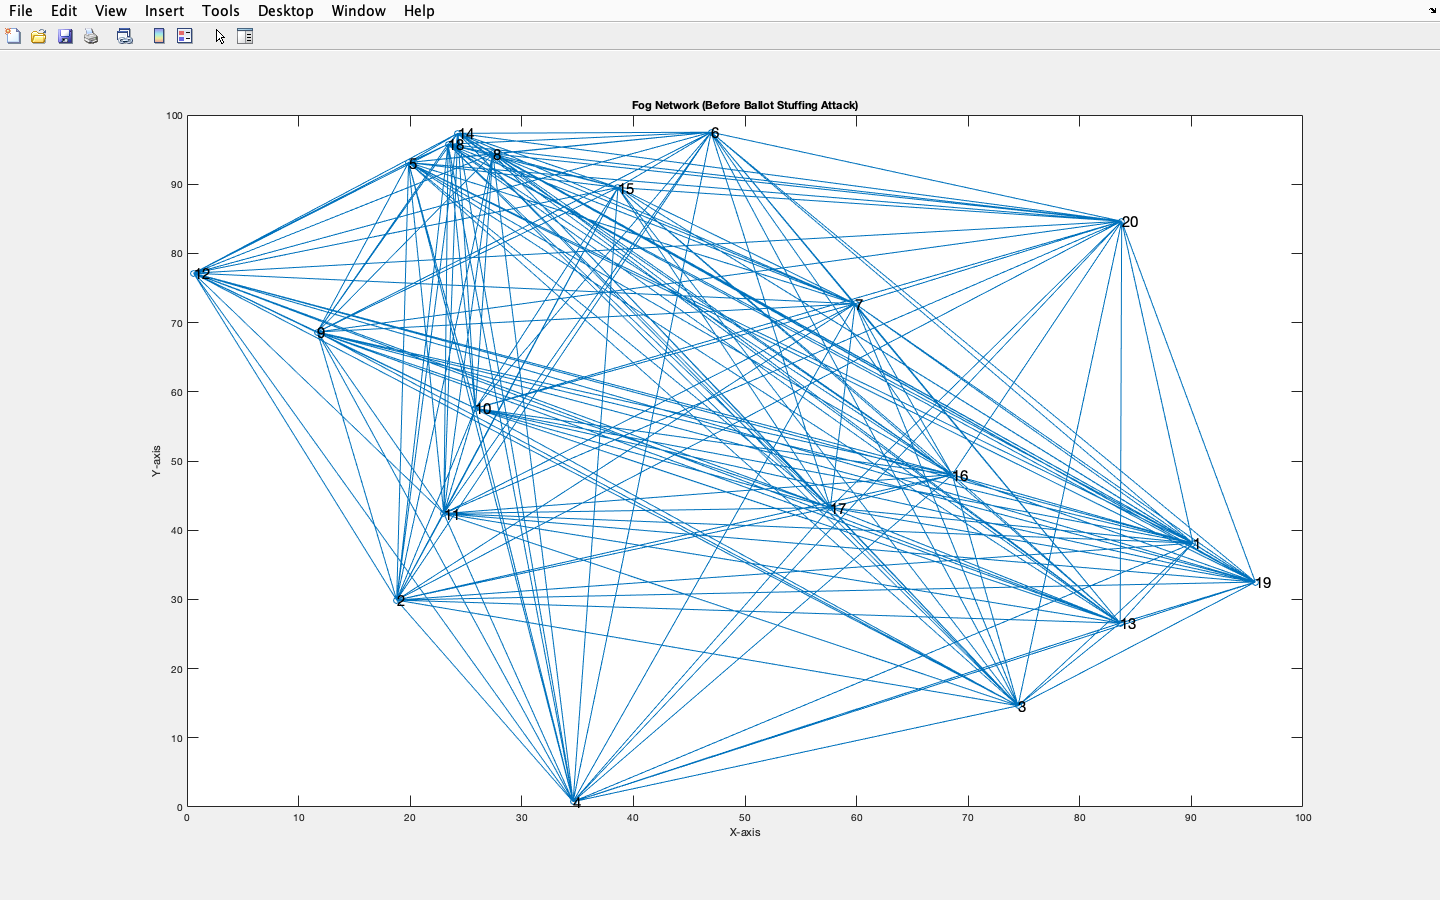
\includegraphics[width=\textwidth]{bst/images/10.png}
        \caption{Interactions among all the 20 fog nodes in the network}
        \label{fig:sub1}
    \end{subfigure}
    \hfill
    \begin{subfigure}[b]{0.8\textwidth}
        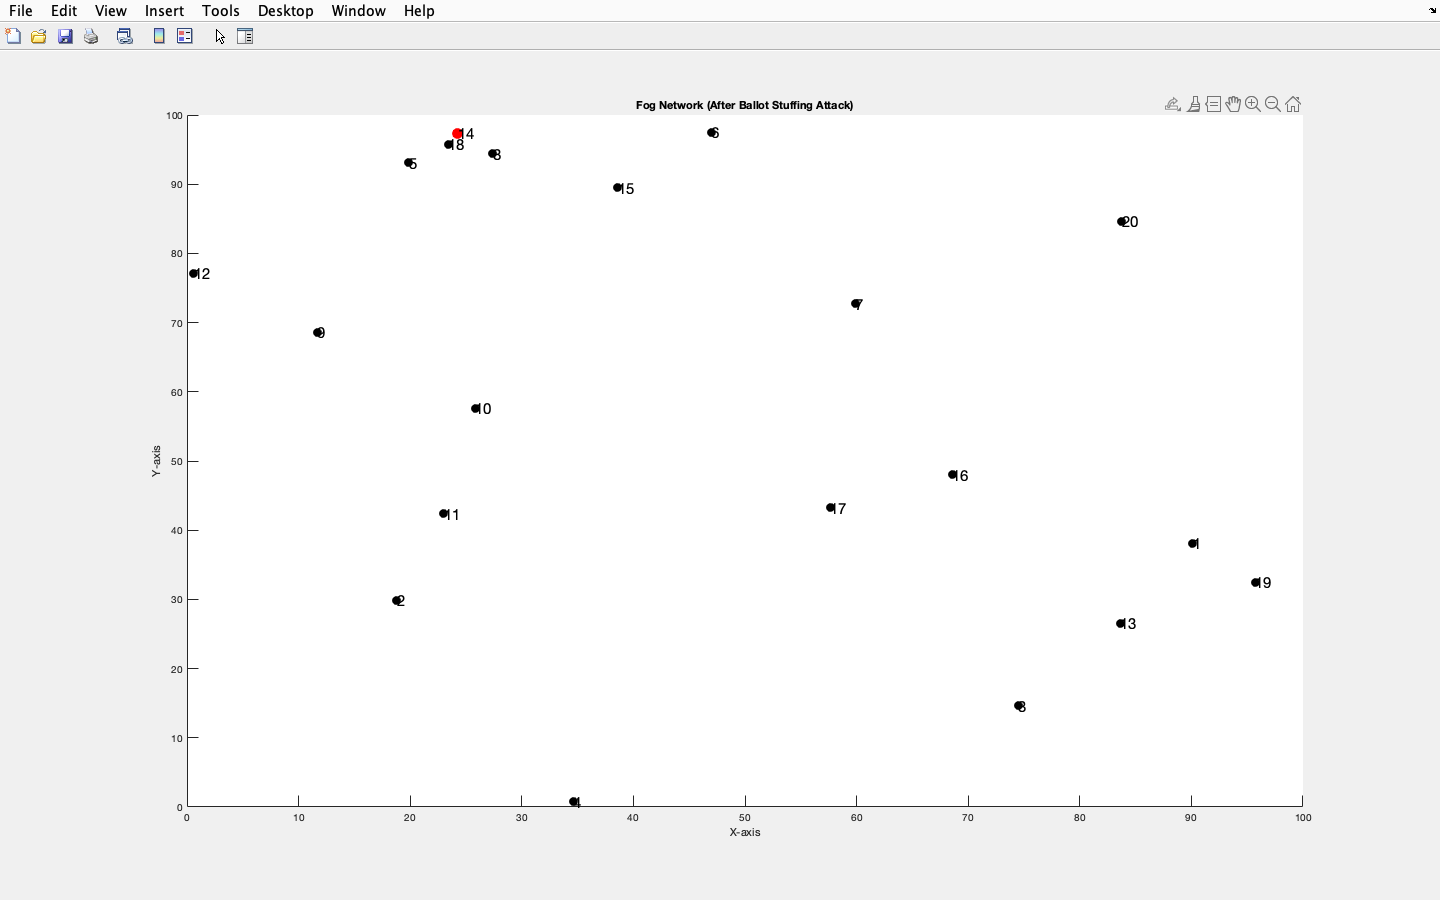
\includegraphics[width=\textwidth]{bst/images/12.png}
        \caption{Identifying N14 (Marked Red) as rogue node post analysis}
        \label{fig:sub2}
    \end{subfigure}
    \caption{Interactions and Detection of Rogue Nodes through Proposed BORTNET Methodology}
    \label{fig:both}
\end{figure*}
\item \textbf{Simulation with 20 Nodes :}
We have also experimented with 20 nodes having a maximum of 6 rogue nodes. Table \ref{tab:total_results_20_nodes} summarizes the borda scores before and after the attack. The rank difference, suspect nodes and finally the suspect scores. As we can observe from the table, N14 is considered as the rogue node which is part of initial assumptions. It is important to note that since the fog manager does not have a count of rogue nodes to be eliminated, the process needs to performed iteratively to remove all the rogue nodes.
\begin{table*}[htbp]
\centering
\caption{Suspect Scores of Each Node}
\label{tab:total_results_20_nodes}
\scalebox{0.8}{
\begin{tabular}{|c|c|c|c|c|c|c|c|c|c|c|}
\hline
Nodes & \makecell{Borda score \\ before attack} & \makecell{Borda score \\ after attack} & \makecell{Rank \\ Difference} & \multicolumn{6}{c|}{Suspect Nodes} & Suspect Score \\
\hline
N1 & 203 & 261 & 7 & 6 & 12 & 8 & 14 & 19 & 5 & 16 \\
\hline
N2 & 187 & 225 & 8 & 17 & 3 & 18 & 5 & 6 & 13 & 21 \\
\hline
N3 & 197 & 235 & 7 & 14 & 1 & 11 & 16 & 20 & 7 & 24 \\
\hline
N4 & 192 & 160 & -8 & 6 & 2 & 14 & 15 & 8 & 18 & 13 \\
\hline
N5 & 163 & 167 & 4 & 8 & 9 & 12 & 2 & 11 & 18 & 22 \\
\hline
N6 & 146 & 166 & 5 & 2 & 9 & 8 & 12 & 15 & 14 & 31 \\
\hline
N7 & 220 & 182 & -9 & 18 & 19 & 14 & 20 & 8 & 11 & 16 \\
\hline
N8 & 168 & 184 & 5 & 13 & 19 & 14 & 15 & 18 & 1 & 45 \\
\hline
N9 & 204 & 194 & -1 & 13 & 5 & 12 & 19 & 14 & 18 & 19 \\
\hline
N10 & 209 & 201 & -1 & 15 & 8 & 5 & 12 & 3 & 16 & 20 \\
\hline
N11 & 182 & 200 & 6 & 4 & 7 & 3 & 9 & 19 & 10 & 27 \\
\hline
N12 & 206 & 204 & 1 & 4 & 5 & 11 & 2 & 20 & 3 & 20 \\
\hline
N13 & 226 & 194 & -8 & 18 & 15 & 8 & 10 & 14 & 19 & 21 \\
\hline
\textbf{N14} & \textbf{210} & \textbf{190} & \textbf{-6} & \textbf{3} & \textbf{19} & \textbf{15} & \textbf{6} & \textbf{17} & \textbf{13} & \textbf{55} \\
\hline
N15 & 167 & 161 & 0 & 0 & 0 & 0 & 0 & 0 & 0 & 33 \\
\hline
N16 & 221 & 229 & -1 & 2 & 18 & 4 & 9 & 11 & 14 & 12 \\
\hline
N17 & 191 & 173 & -2 & 11 & 20 & 10 & 7 & 8 & 2 & 16 \\
\hline
N18 & 180 & 162 & -2 & 12 & 6 & 9 & 11 & 17 & 3 & 44 \\
\hline
N19 & 153 & 155 & -1 & 8 & 9 & 7 & 11 & 13 & 4 & 42 \\
\hline
N20 & 175 & 157 & -4 & 4 & 10 & 14 & 16 & 1 & 5 & 19 \\
\hline
\end{tabular}
}
\end{table*}
Simulation of node interactions and identification of N14 as rogue node can also be observed from the simulated matlab environment depicted in Fig. \ref{fig:sub1}.




To ensure the ongoing security and reliability of the network, this analytical procedure should be periodically repeated. Consistent monitoring and reevaluation are crucial for identifying emergent threats or behavioral anomalies among the nodes. A network exhibiting no significant rank differences over time is indicative of stability and absence of internal disruptions. Conversely, the appearance of rank differences signals potential security breaches or attacks, necessitating immediate investigative and corrective actions. It can observed that this approach is robust and also scalable which is important for a for environment.

 
\end{itemize}

\section{Conclusion}

The proposed methodology, implemented and tested in a fog computing environment, effectively identifies rogue nodes through the computation of trust matrices and the analysis of voting discrepancies. The experimental results demonstrated the robustness of the trust matrix generation, employing a star topology where nodes communicated in a simulated setting with dynamic trust adjustments based on the outcomes of these interactions. This foundational step allowed us to capture the essential trust relationships within the network accurately.

Subsequent phases of the methodology leveraged these trust matrices to detect anomalies in node behavior through a sophisticated analysis of voting matrices, further refined by comparing original and manipulated rankings. The detection process was validated using a hypothetical scenario involving rogue nodes, which manipulated rankings to disrupt network integrity. Our approach successfully identified these nodes by calculating discrepancies in rankings and applying a scoring system that quantified the impact of each node's actions on the network's trustworthiness.

This systematic identification and scoring mechanism significantly contribute to the field of fog computing security, providing a scalable and efficient method to maintain network integrity. By adhering to the principles of Byzantine fault tolerance, our methodology ensures that the network can sustain a limited number of rogue nodes without compromising its overall functionality.

\subsection{Future Directions}

Moving forward, there are several avenues for enhancing this research. Firstly, integrating machine learning techniques to predict node behavior based on historical data could provide preemptive security measures, potentially stopping attacks before they start. Additionally, exploring the application of blockchain technology could offer a decentralized and transparent method for managing trust and voting records, further securing the network against tampering.

Another promising direction involves extending the methodology to more complex network topologies and larger scales, which would test the robustness and scalability of the current approach in more dynamic and unpredictable environments. Finally, conducting real-world tests in commercial fog computing networks would provide valuable insights into the practical challenges and performance implications of implementing such security measures. These enhancements and expansions could significantly improve the resilience of fog computing networks, ensuring their reliability and security in the face of evolving cyber threats.







\subsection *{Declarations}

\begin{itemize}
    \item []\textbf{Ethical approval :} This article does not contain any studies with human participants performed by the authors.

    \item[] \textbf{Conflict of interest :}  We want to confirm that there are no known conflicts of interest linked with this publication. 
    
\item[] \textbf{Competing Interests :} We declare that the there are no competing interests or other interests that might be perceived to influence the results and/or discussion reported in this paper.

\item[]\textbf{Author's contributions :}
We check that all named authors read and approved the article and that there are no other people who met the criteria for authorship but are not included. We also affirm that all have agreed the authorship order indicated in the manuscript of us.

\item[] \textbf{Funding :} No significant financial assistance for this work has been provided that could have influenced its outcome.

\item[] 
\textbf{Data Availability :} No datasets were used for this work.

    
\end{itemize}




%%===========================================================================================%%
%% If you are submitting to one of the Nature Portfolio journals, using the eJP submission   %%
%% system, please include the references within the manuscript file itself. You may do this  %%
%% by copying the reference list from your .bbl file, paste it into the main manuscript .tex %%
%% file, and delete the associated \verb+\bibliography+ commands.                            %%
%%===========================================================================================%%

% \bibliography{references}% common bib file
% \bibliography{references}
\bibliographystyle{plain}  
\bibliography{main}  

%% if required, the content of .bbl file can be included here once bbl is generated
%%\input sn-article.bbl






\end{document}
